\let\negmedspace\undefined
\let\negthickspace\undefined
\documentclass[journal]{IEEEtran}
\usepackage[a5paper, margin=10mm, onecolumn]{geometry}
\usepackage{lmodern} % Ensure lmodern is loaded for pdflatex
\usepackage{tfrupee} % Include tfrupee package

\setlength{\headheight}{1cm} % Set the height of the header box
\setlength{\headsep}{0mm}     % Set the distance between the header box and the top of the text

\usepackage{gvv-book}
\usepackage{gvv}
\usepackage{cite}
\usepackage{amsmath,amssymb,amsfonts,amsthm}
\usepackage{algorithmic}
\usepackage{graphicx}
\usepackage{textcomp}
\usepackage{xcolor}
\usepackage{txfonts}
\usepackage{listings}
\usepackage{enumitem}
\usepackage{mathtools}
\usepackage{gensymb}
\usepackage{comment}
\usepackage[breaklinks=true]{hyperref}
\usepackage{tkz-euclide} 
\usepackage{listings}                                      
\def\inputGnumericTable{}                                 
\usepackage[latin1]{inputenc}                                
\usepackage{color}                                            
\usepackage{array}                                            
\usepackage{longtable}
\usepackage{multicol}
\usepackage{calc}                                             
\usepackage{multirow}                                         
\usepackage{hhline}                                           
\usepackage{ifthen}                                           
\usepackage{lscape}
\begin{document}

\bibliographystyle{IEEEtran}
\vspace{3cm}

\title{12.6.5.3.4}
\author{EE24BTECH11010 - Balaji B}
% \maketitle
% \newpage
% \bigskip
{\let\newpage\relax\maketitle}

\renewcommand{\thefigure}{\theenumi}
\renewcommand{\thetable}{\theenumi}
\setlength{\intextsep}{10pt} % Space between text and floats


\numberwithin{equation}{enumi}
\numberwithin{figure}{enumi}
\renewcommand{\thetable}{\theenumi}


\textbf{Question}:\\
Find the local maximum and local minimum values of the function $f(x) = \sin{x} - \cos{x}$ for $x$ the interval $\sbrak{0,2\pi}$ .

\textbf{Theoretical Solution:}\\
To find critical points, we equalize $\frac{df(x)}{dx}$ = 0. Let $y = f(x)$
\begin{align}
\frac{dy}{dx} &= \cos{x} + \sin{x} \\
 \cos{x} + \sin{x} &= 0 \\
 \tan{x} &= -1
\end{align}
For $x \in \sbrak{0,2\pi}$ , $\tan{x} = -1$ for $x = \frac{3\pi}{4}$ and $\frac{7\pi}{4}$.\\\\
To find maxima and minima, we should double the derivative of the function $f(x)$. On double derivating we get,
\begin{align}
    \frac{d^2y}{dx^2} = \cos{x} - \sin{x}
\end{align}
On applying the critical point $x = \frac{3\pi}{4}$, we get
\begin{align}
    \frac{d^2y}{dx^2} = -\sqrt{2}
\end{align}
As the double derivative is negative at $x = \frac{3\pi}{4} $, so we have maxima at that point.\\\\
Similarly, when we apply the critical point $x = \frac{7\pi}{4}$, we get
\begin{align}
\frac{d^2y}{dx^2} = \sqrt{2}
\end{align}
As the double derivative is positive at $x = \frac{7\pi}{4} $, so we have minima at that point.\\
$\therefore$ Local maxima at $x = \frac{3\pi}{4}$

 Local minima at $x = \frac{7\pi}{4}$\\
 
\textbf{Computational Solution: }\\
We use the gradient descent method to find the local maximum and local minimum of the given function.
\begin{align}
    f^\prime\brak{x_{n}} &= \cos{\brak{x_{n}}} + \sin\brak{{x_n}}
\end{align}
Gradient decent to find local minimum
\begin{align}
x_{n+1} &= x_{n} - \eta f^\prime\brak{x_{n}} \\
    x_{n+1} &= x_{n} - \eta \brak{\cos{\brak{x_{n}}} + \sin{\brak{x_n}}}
\end{align}
Gradient ascent to find local maximum,
\begin{align}
    x_{n+1} &= x_{n} + \eta f^\prime\brak{x_{n}} \\
    x_{n+1} &= x_{n} + \eta \brak{\cos{\brak{x_{n}}} + \sin{\brak{x_n}}}
\end{align}
Where $\eta$ is the learning rate.

Assuming,
\begin{align}
    \eta &= 0.1 \\
    \text{tolerance} &= 1e-6 \\
    x_{0} &= 0.0
\end{align}
We get,
\begin{align}
    x_{min} = 2.356194 &,\quad y_{min} = 1.414214 \\
    x_{max} = 5.497788 &,\quad y_{max} = -1.414214
\end{align}
\newpage

\begin{figure}[ht]
    \centering
    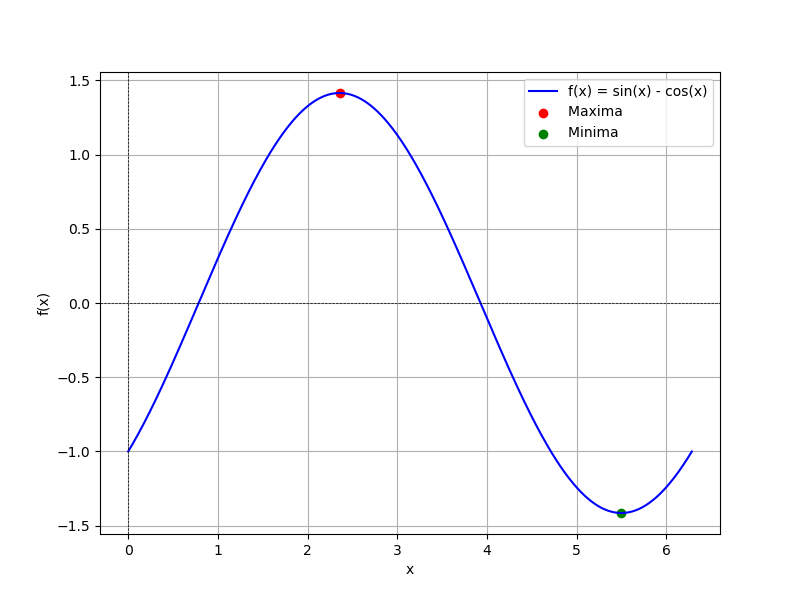
\includegraphics[width=\columnwidth]{figs/fig.png}
    \caption{Plot of local maximum and minimum}
    \label{fig:Plot1}
    \end{figure}
\end{document}}
